\chapter{系统实现说明}
\label{chap:2}

本章重点在于说明运用技术的调研与说明目前主流可用方案,同时讲述系统规划。

\section{系统开发平台考量}

本作业在规划时考虑过在不同平台与不同方式开发的可行性方案,在应用程式开发上,若选择桌面开发可以使用 PyQt,而对应的行动装置上则可使用 React Native 使用 JS 技术开发完后,转成行动装置的 APP。

而使用网页技术开发,则考量可以运用 Web 的前后端开发,先完成桌面的应用跟规划后,再根据响应式网页的方式,将原有的桌面功能转为行动端的功能。而在此使用 Python Flask 与前端框架。

\begin{figure}[htb]
\centering 
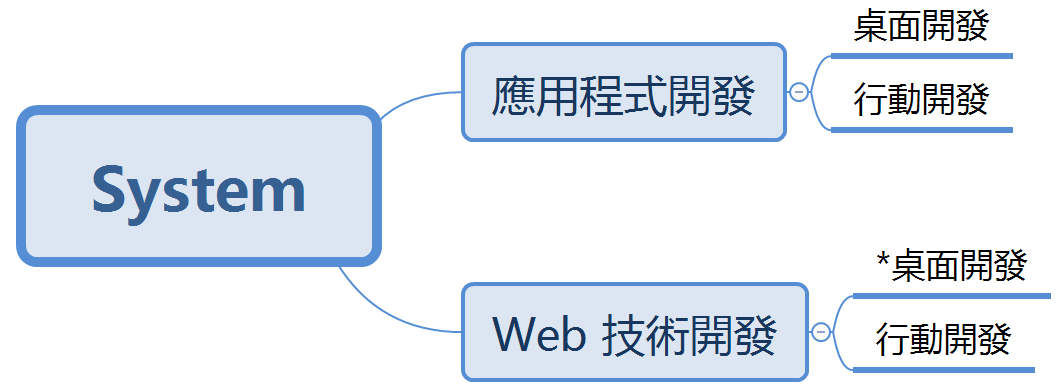
\includegraphics[width=0.80\textwidth]{img/ch2m0.png} 
\caption{系统开发方案}
\label{Test}
\end{figure}


%\begin{itemize}
%\item [-] L1
%\end{itemize}

\section{技术调研}

此节将本次作业所考量的技术与方案逐一进行说明,當中包含了前端框架、后端方案、应用程式方案與深度学习框架。

\subsection{前端框架}

在此作业中考量过三大前端的主流框架,分别是 Vue、Google 主导的 Angualr 框架与 脸书主导的 React 框架,根据开发的容易程度与开发团队的适应性,本作业最终选择了 Vue。其 Vue 的开发者尤雨溪开发出了此框架。他声称自己的思路是提取 Angular 框架中中为自己所喜欢的部分,从而构建而出。而当中三个框架的环境部属等指令如下。

\begin{Verbatim}
# Vue
# 安装 CLI
$ npm install --global @vue/cli

# VUE 版本
$ vue --version

# 建立 Vue 专案
$ vue create vue-app

# 伺服器执行
$ npm run serve

# Angualr
# 安装 CLI
$ npm install -g @angular/cli

# 建立 Angular 专案
$ ng new ag-app

# 进入专案
$ cd ag-app

# 启动 Server
$ ng serve --open

# React
$ npm install -g create-react-app

# 建立名为 react-app 的 React 专案
$ create-react-app react-app

$ create-react-app [Project Name]

# 进入 React 专案执行
$ npm start

\end{Verbatim}

\subsection{后端方案}

其原本有 Python、GO、PHP 的 Laravel 与 Java 的 Spring Boot 框架 择一进行开发,原因在于再开发应用程式或者后端开发,这些技术都已经相当成熟,在该技术的使用者上多。比如很多在人脸辨识等可商业化用途的平台是用 Java 为开发基础,同时 Go 也有现有的开源串流与版本控制方案,再之后开发可以考虑系统整合。

最后则是 Python,目前有两个主流开发方案,一个是 Python Flask,另一个是 Python Django,前者专注于轻量化的发展,面对简易的伺服器服务,而后者则针对庞大的服务支援发展许久。同时 Python 不同领域也有很多的发展,比如网页自动化测试、人脸辨识、应用程式开发、数据分析、深度学习等等,况且此次作业需要整合深度学习的框架,故本次作业选择使用 Python Flask 进行开发。而当中 Python Flask 在安装相对套件后,简易 Demo 如下可见,如执行成功可以于预设本地端 5000 Port ,看到网页上输出字串为 OwO//。另外 Python Django 与 Python Flask 环境安装的指令如下所示。

1. Python Django 环境部署

\begin{Verbatim}
# Python 版本
> py -3 -V

# Pip 安装的所有套件资讯
> pip3 list

# 安装
> pip install virtualenv
> pip install virtualenvwrapper-win

# 执行
> mkvirtualenv my_django_environment
> virtualenv test

# 安装 Django
> pip3 install django

# Django 版本
> py -3 -m django --version

# 建立 Django 目录
> mkdir django_test
> cd django_test

# 建立 Django 专案
> django-admin startproject mytestsite
> cd mytestsite

# 执行 Django Server
> py -3 manage.py runserver
\end{Verbatim}

2. Python Flask 环境部署

\begin{Verbatim}
pip install flask-socketio
pip install flask-wtf
pip install eventlet
pip install gevent
\end{Verbatim}

3. Python Flask 执行

\begin{Verbatim}
from flask import Flask

app = Flask(__name__)

@app.route("/")
def home():
    return "OwO//"

app.run()
\end{Verbatim}



\subsection{应用程式方案}

此节针对前一节所述,由于 Python 在广泛的领域都有着不俗的应用,在此应用程式的开发上,本作业预设考量为 PyQt 其方案为 Python 语言的 GUI 解决方案之一,可以用来代替 Python 中内建的 Tkinter,另外 PyQt 的开发者为英国的 Riverbank Computing 公司,该公司提供了 GPL 与商业协定两种授权方式,因此它可以免费地用于自由软体的开发。当中 PyQt 的执行如下,执行完后可以看到一个视窗上出现 Hello, World! OwO // 的文字。

\begin{Verbatim}
class MyWidget(QWidget):
    def __init__(self):
        super().__init__()
        self.initUI()

    def initUI(self):
        self.setWindowTitle('Window')
        self.setGeometry(150, 150, 400, 350)

        self.mylabel = QLabel('Hello, World! OwO //', self)
        self.mylabel.move(60, 50)

if __name__ == '__main__':
    app = QApplication(sys.argv)
    w = MyWidget()
    w.show()
    sys.exit(app.exec_())
\end{Verbatim}


\subsection{深度学习方案}

本作业考量的深度学习方案有两个,其一为由脸书所主导的 PyTorch ,其二为 Google 所主导的 TensorFlow,但由于近年来 PyTorch 本作业的开发成员熟悉度较高,本作业选择采用 PyTorch 为开发方案。而在此将环境建立 Tensorflow, Keras, PyTorch 的指令如下所示。

\begin{Verbatim}
# 建立工作目录
> md \pythonwork
> cd \pythonwork

# 使用 conda 命令来建立一个命名为 tensorflow 的虚拟环境,并在里面安装 Python 3.8 版本
# Python 版本根据 Anaconda 安装的版本而定
# 基本上名字任意,当下命名为 tensorflow
> conda create --name tensorflow python=3.8

# 利用activate tensorflow 命令启动 tensorflow 的 anaconda 虚拟环境
# 若要关闭虚拟环境则是使用 deactivate tensorflow
# To activate this environment, use
> conda activate tensorflow

# To deactivate an active environment, use
> conda deactivate

# 检视当下环境状态
> conda info -e

# conda 版本
> conda --version

# 安装 Tensorflow
> conda install tensorflow

# 安装 Keras
> conda install -c conda-forge keras

# 在被命名成 tensorflow 的虚拟环境底下安装 jupyter notebook
> conda activate tensorflow

# 处理前面会有 (tensorflow) 开头
> conda install jupyter notebook

# 安装 PyTorch
> conda install pytorch torchvision cpuonly -c pytorch

# Jupyter Notebook 执行 Tensorflow, Keras, PyTorch

# Tensorflow
import tensorflow as tf
import tensorflow.compat.v1 as tf
hello = tf.constant("Hello, TensorFlow!")
sess = tf.compat.v1.Session()
print(sess.run(hello))

# Keras
from keras import datasets
# Load MNIST data
(train_images, train_labels), (test_images, test_labels) = datasets.mnist.load_data()
# Check the dataset loaded
train_images.shape, test_images.shape

# PyTorch
import torch
print(torch.__version__)
\end{Verbatim}


%\begin{figure}[htb]
%\centering 
%\includegraphics[width=0.60\textwidth]{img/picname.png} 
%\caption{XXXX}
%\label{Test}
%\end{figure}
